\documentclass[
a4paper, % Paper size, use either a4paper or letterpaper
12pt, % Default font size, the template is designed to look good at 12pt so it's best not to change this
%unnumberedsections, % Uncomment for no section numbering
]{SourcesTemplate/TemplateReport}

%----------------------------------------------------------------------------------------
%	REPORT TILE INFORMATION
%----------------------------------------------------------------------------------------

\confidentielfalse % Print confidentiel in the main page, comment it to remove it 

\reporttitle{Synthèse de champ sonore diffuse} % The report title
\reportshorttitle{ \reporttitle} % The report short title  to change in case of too long title
\reportsubtitle{ } 

\reportauthors{Samuel Dupont \\\href{mailto:Samu.dupont@laposte.net}{Samu.dupont@laposte.net}

} % Report authors/group/department, include new lines if needed

\reportdate{\today} % Report date, include new lines for additional information if needed

\leftheadercontent{} % if not empty with a path toward a img, replace deafult logo in the left header

%----------------------------------------------------------------------------------------
%	Fiche signaletique  INFORMATIONS
%----------------------------------------------------------------------------------------
\refdoc{ARL/RT/??-??}
\refcommand{ SystemGIE ?? du 03/03/2023 \newline 		Référence ?? : ??} 
\refprop{PTC00?? du ??/??/??} 

\newcommand{\organismeDestinatairesList}{%
	% Add more pairs as needed
	\addOrganismeDestinatairesPairs{Your Organization}{Recipient 1}%
	\addOrganismeDestinatairesPairs{Another Organization}{Recipient A}%
}

\newcommand{\versionTripletList}{%
	% Add more triplet as needed
	\addVersionTriplet{2023-01-01}{0}{4}%
	\addVersionTriplet{\reportdate}{1}{\pageref{LastPage}}%
}

\redacteur{John Doe}
\verificateur{Jane Smith}
% Define a variable to store the list of pairs

\begin{document}

% make front page 
\makefrontpage{\classfolder/images_cls/logo_neutral.png}

% make fiche signaletique 

\tableofcontents % This command generates the table of contents


\chapter{Introduction}

\section{Contexte}

\section{Formulation du champ diffus}
\begin{equation}
	\hat{p}_{tot} = \sum_{q}	\hat{p}_q e^{ik\mathbf{n}_q.\mathbf{x}}
\end{equation}
\begin{equation}
	\rho c \mathbf{\hat{v}}_{tot} = \sum_{q} \mathbf{n}_q \hat{p}_q e^{ik\mathbf{n}_q.\mathbf{x}}
\end{equation}
% TODO: \usepackage{graphicx} required
\begin{figure}
	\centering
	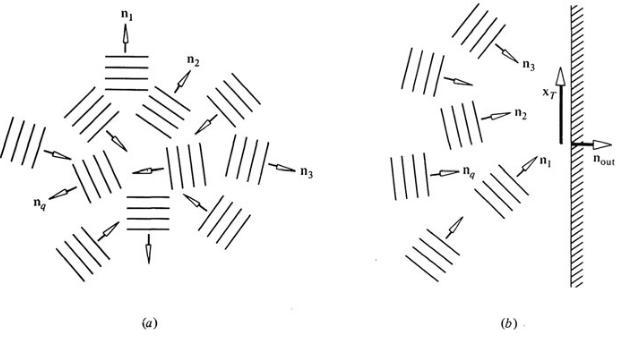
\includegraphics[width=0.7\linewidth]{images/planew}
	\caption{(a) Reverberant field represented as a superposition of traveling plane waves. (b)Waves incident on a surface adjacent to a reverberant field, \cite{pierce_acoustics_2019}}
	\label{fig:planew}
\end{figure}

A diffuse field can be taken as a superposition of many plane waves. It involves a double sum over indices q and q′,but the process of taking a local spatial average causes the cross terms (q = q′)to average out. The spatial average of $e^{ik(\mathbf{n}_q-\mathbf{n}_q ) . \mathbf{x}}$ is nearly zero for a sufficiently large averaging volume.
\begin{equation}
\begin{split}
	 2* \rho c I & =\sum_{q, r}  \hat{p}_q  \hat{p}_r^* e^{ik(\mathbf{n}_q\mathbf{n}_r).\mathbf{x}^T} \mathbf{n}_r.\mathbf{n}_{out}\\
	& = \sum_{q, r, q\neq r}  \hat{p}_q  \hat{p}_r^* e^{ik(\mathbf{n}_q-\mathbf{n}_r).\mathbf{x}^T} \mathbf{n}_r.\mathbf{n}_{out} + \sum_{q}  \hat{p}_q  \hat{p}_q^*  \mathbf{n}_r.\mathbf{n}_{out}\\
	\end{split}
\end{equation}

\section{Definition de l'absorption diffuse}
If many plane waves are simultaneously incident on a wall, the individual waves reflect independently and the principle of superposition can be used in conjunction with the theory of plane-wave reflection. Such an analysis requires that the time average of the rate at which energy is absorbed (not reflected) by the surface per unit area be : 

\begin{equation}
	\frac{1}{2\rho c}\Re \left\{ pv^*\right\}
\end{equation}
\begin{equation}
	\frac{1}{2\rho c}\Re \left\{  \sum_{q, r}  \hat{p}_q  \hat{p}_r^*(1+R_q)(1-R_q^*) e^{ik(\mathbf{n}_q-\mathbf{n}_r).\mathbf{x}^T} \mathbf{n}_r.\mathbf{n}_{out}\right\}
\end{equation}
the sum is restricted to incident waves, such that nr points obliquely toward the wall.
Inside the parenthesis we have : 
\begin{equation}
	\frac{1}{2\rho c}\Re \left\{  \sum_{q, r}  \hat{p}_q  \hat{p}_r^*(1+R_q)(1-R_q^*) e^{ik(\mathbf{n}_q-\mathbf{n}_r).\mathbf{x}^T} \mathbf{n}_r.\mathbf{n}_{out}\right\}
\end{equation}
\begin{equation}
	\begin{split}
  &\sum_{q, r}  \hat{p}_q  \hat{p}_r^*(1+R_q)(1-R_q^*) e^{ik(\mathbf{n}_q-\mathbf{n}_r).\mathbf{x}^T} \mathbf{n}_r.\mathbf{n}_{out} \\
  &=  \sum_{q, r, q\neq r}  \hat{p}_q  \hat{p}_r^* e^{ik(\mathbf{n}_q-\mathbf{n}_r).\mathbf{x}^T} \\
  &+ \sum_{q, r, q\neq r} R_q \hat{p}_q  \hat{p}_r^* e^{ik(\mathbf{n}_q-\mathbf{n}_r).\mathbf{x}^T} \\
  & -\sum_{q, r, q\neq r} {R}_q^* \hat{p}_q  \hat{p}_r^* e^{ik(\mathbf{n}_q-\mathbf{n}_r).\mathbf{x}^T} \\
  &+ \sum_{q, r, q\neq r} {R}_q^*R_q \hat{p}_q  \hat{p}_r^* e^{ik(\mathbf{n}_q-\mathbf{n}_r).\mathbf{x}^T} \\
&- \sum_{q, q} \left|p_q\right|^2  (1+R_q - R_q^*-\left|R_q^2\right|)  \\
	\end{split}
\end{equation}
Considering that the spatial average of $e^{ik(\mathbf{n}_q-\mathbf{n}_q ) . \mathbf{x}}$ is nearly zero for a sufficiently large averaging volume.
\begin{equation}
	\begin{split}
		&\sum_{q, r}  \hat{p}_q  \hat{p}_r^*(1+R_q)(1-R_q^*) e^{ik(\mathbf{n}_q-\mathbf{n}_r).\mathbf{x}^T} \mathbf{n}_r.\mathbf{n}_{out} \\
		&= \sum_{q, q} \left|p_q\right|^2  (1+R_q - R_q^*-\left|R_q^2\right|) \\
	\end{split}
\end{equation}
Then by taking the real part :
\begin{equation}
		\begin{split}
		&	\frac{1}{2\rho c}\Re \left\{  \sum_{q, r}  \hat{p}_q  \hat{p}_r^*(1+R_q)(1-R_q^*) e^{ik(\mathbf{n}_q-\mathbf{n}_r).\mathbf{x}^T} \mathbf{n}_r.\mathbf{n}_{out}\right\} \\ \\
		&=	\frac{1}{2\rho c} \sum_{q, q} \left|p_q\right|^2  (1-\left|R_q^2\right|) \mathbf{n}_r.\mathbf{n}_{out} \\
	\end{split}	
\end{equation}

The diffuse field alpha can thus be obtain from : à revoir
\begin{equation}
\alpha_\text{diff} = \frac{{\Re}\left(\sum pv^*\right) z_0}{\sum\left|p_q\right|^2 2 \cos \phi}
\end{equation}

\section{Analyse des termes diagonaux}
SImulation en plane wave uniquement, sur un plan de microphones pour l'average spatial. La pression et la vitesse sont calculés dessus. \\
\textbf{Proof exemple : }10 PW, 2000 Microphones réparties sur une large zone 10000 m ( spatial average)\\

	\begin{figure}[h!]
	\captionsetup{width=0.45\textwidth}
	\begin{minipage}[c]{.45\linewidth}
		\begin{center}
	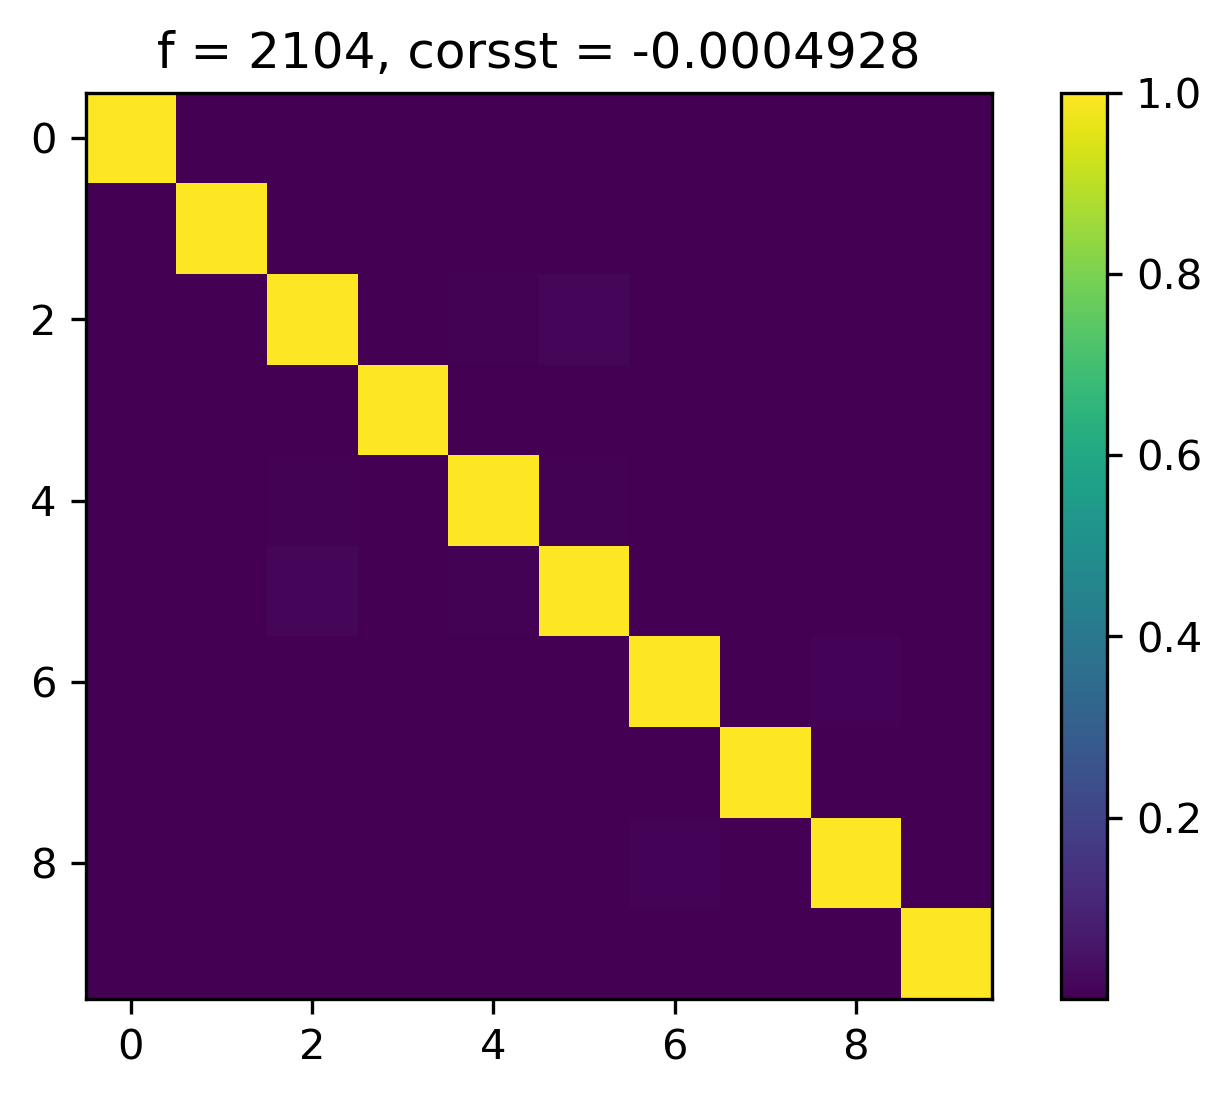
\includegraphics[width=0.9\linewidth]{images/cross1}
			\caption*{Plane wave matrix correlation}
		\end{center}
	\end{minipage}
	\hfill
	\begin{minipage}[c]{.45\linewidth}
		\begin{center}
	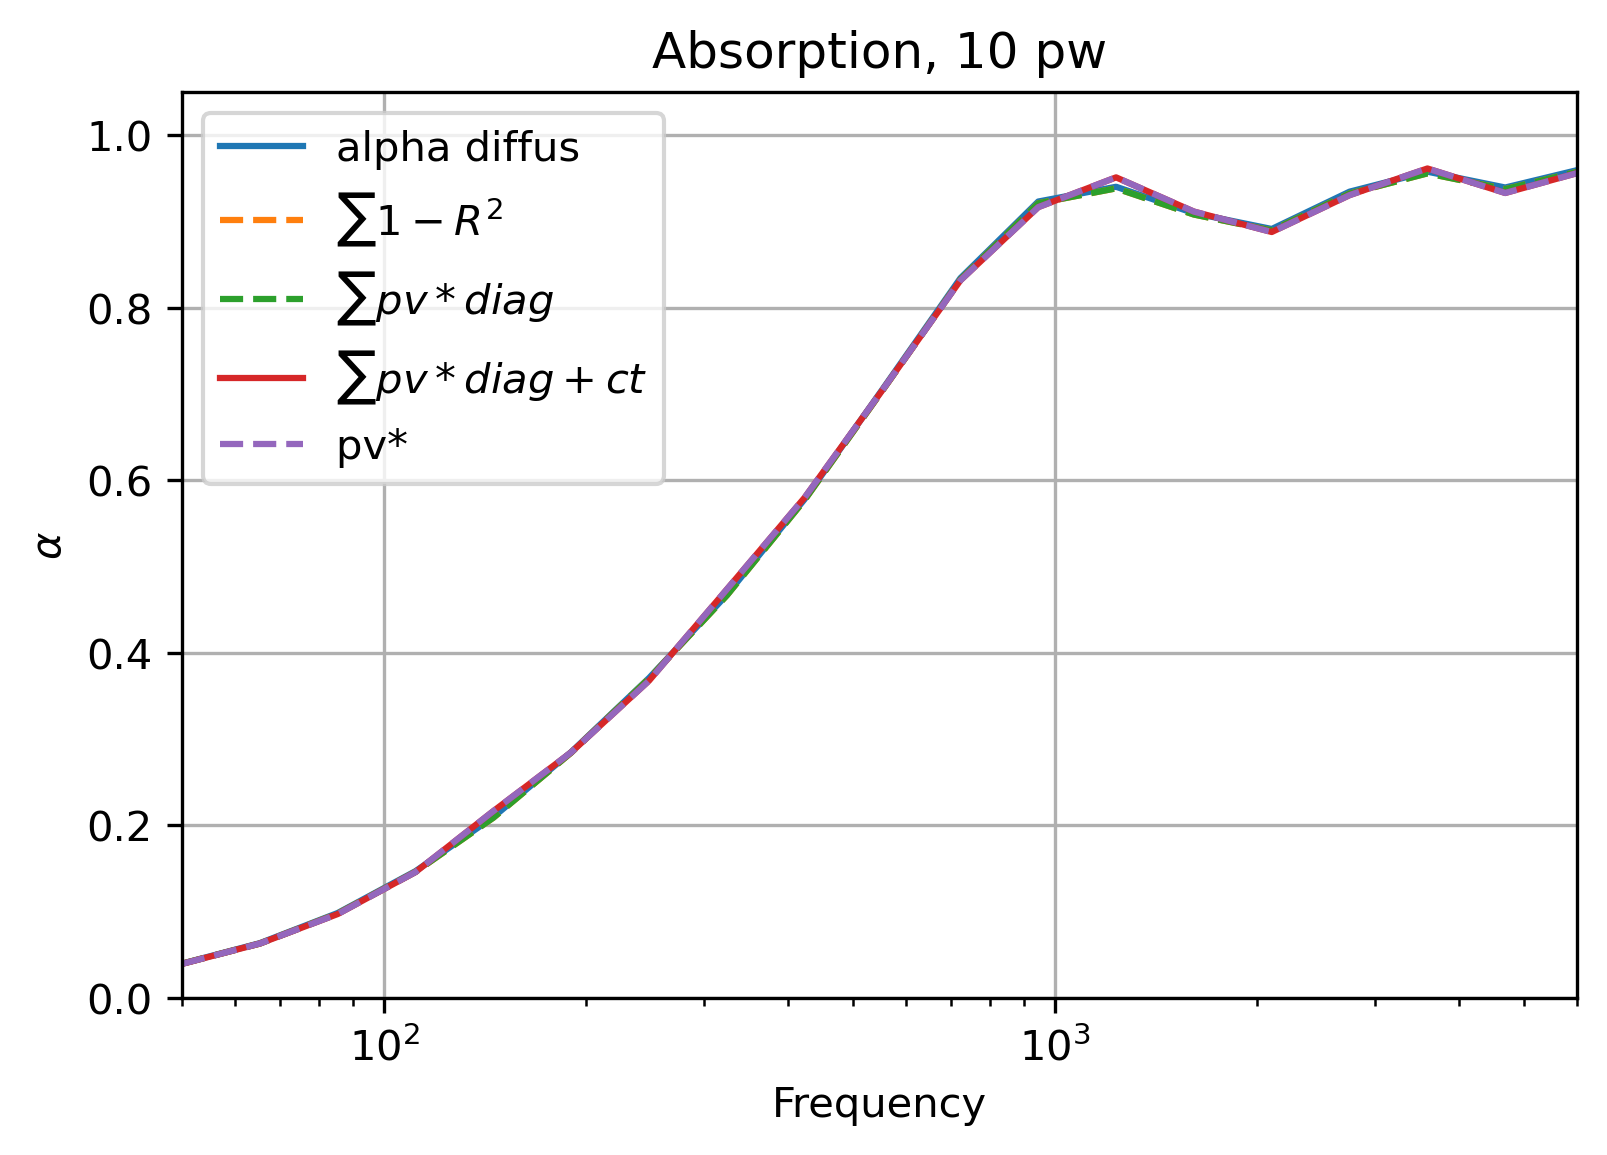
\includegraphics[width=0.9\linewidth]{images/cross2}
			\caption*{Corresponding absorption}
		\end{center}
	\end{minipage}
\end{figure}	
	
\textbf{Exemple : }10 PW, 200 Microphones réparties sur une large zone 10000 m ( spatial average)\\

\begin{figure}[h!]
	\captionsetup{width=0.45\textwidth}
	\begin{minipage}[c]{.45\linewidth}
		\begin{center}
			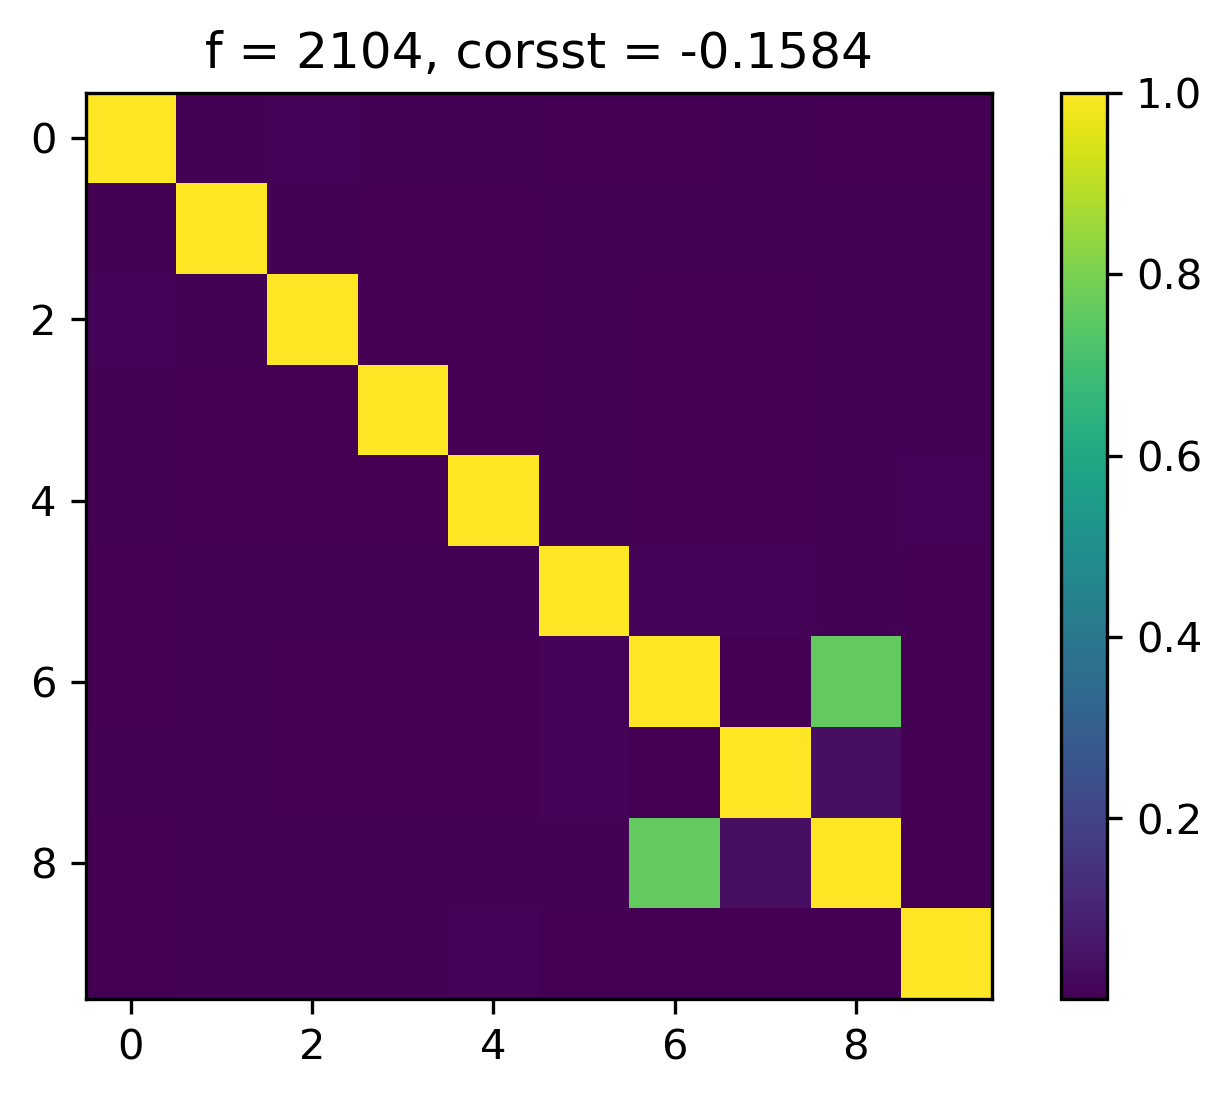
\includegraphics[width=0.9\linewidth]{images/cross3}
			\caption*{Plane wave matrix correlation}
		\end{center}
	\end{minipage}
	\hfill
	\begin{minipage}[c]{.45\linewidth}
		\begin{center}
			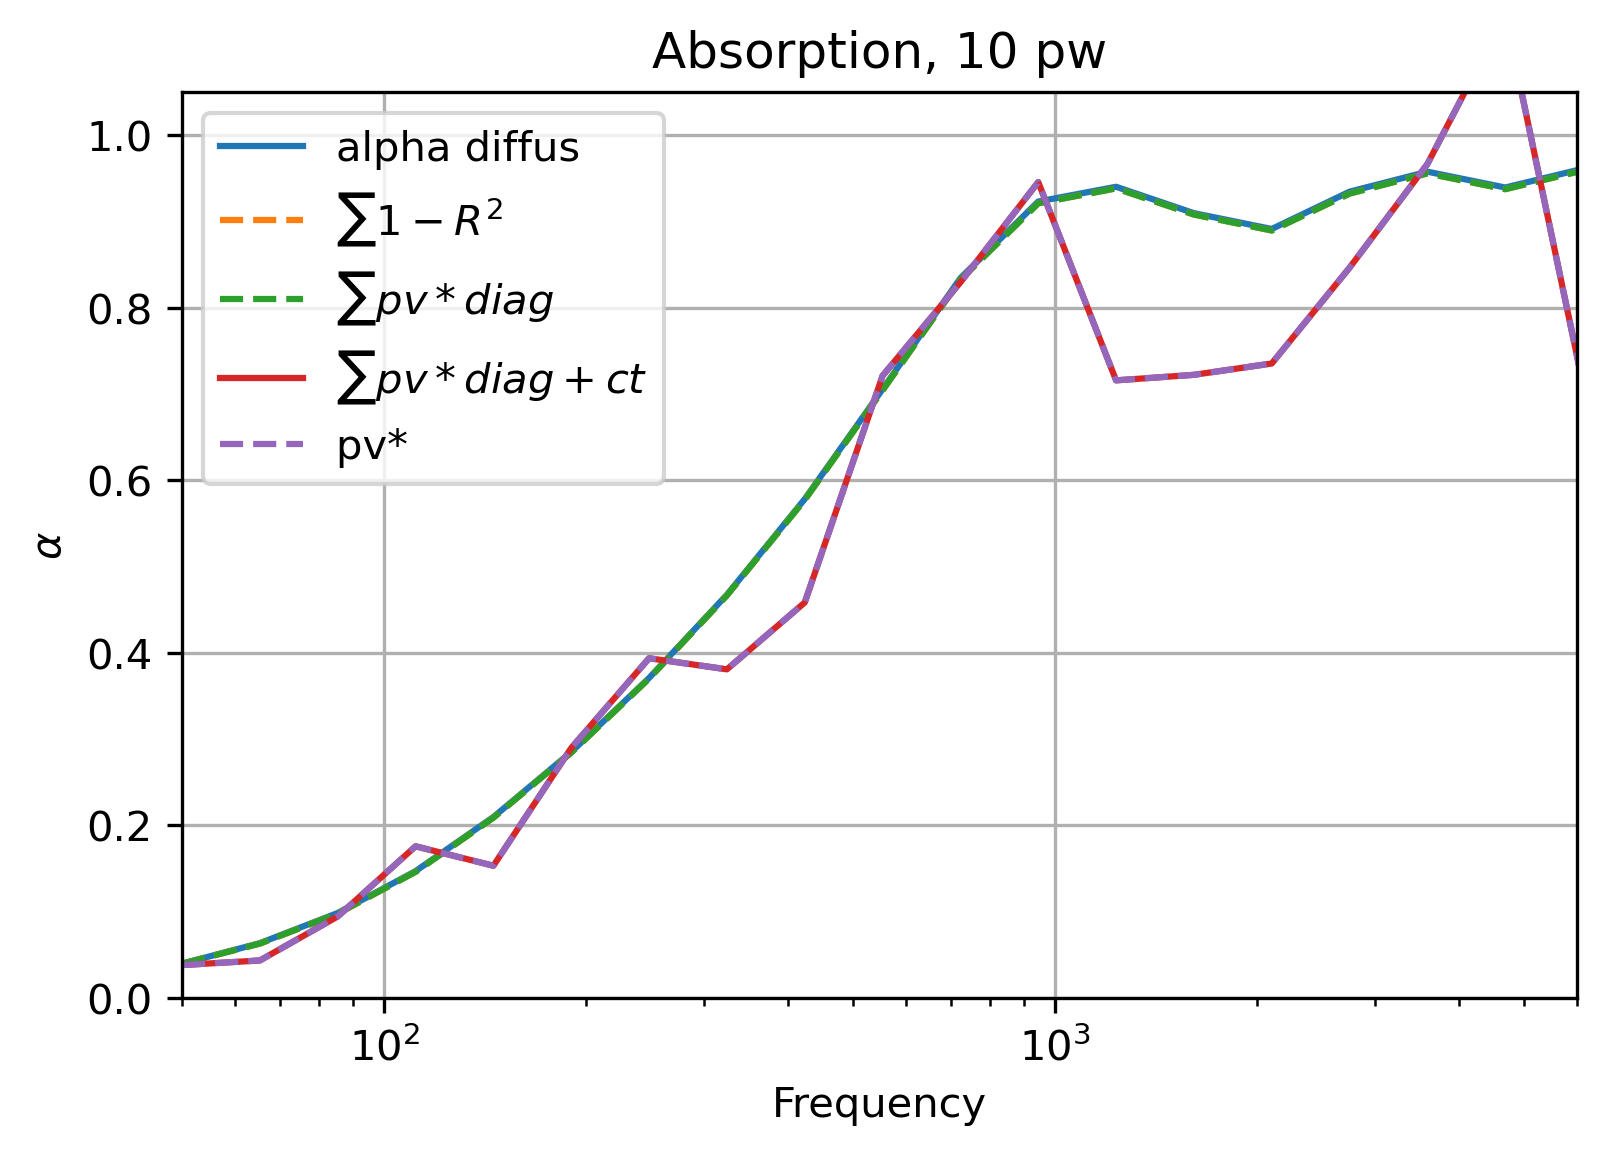
\includegraphics[width=0.9\linewidth]{images/cross4}
			\caption*{Corresponding absorption}
		\end{center}
	\end{minipage}
\end{figure}	
	
\textbf{Exemple : }100 PW, 200 Microphones réparties sur une large zone 10000 m ( spatial average)\\

\begin{figure}[h!]
	\captionsetup{width=0.45\textwidth}
	\begin{minipage}[c]{.45\linewidth}
		\begin{center}
			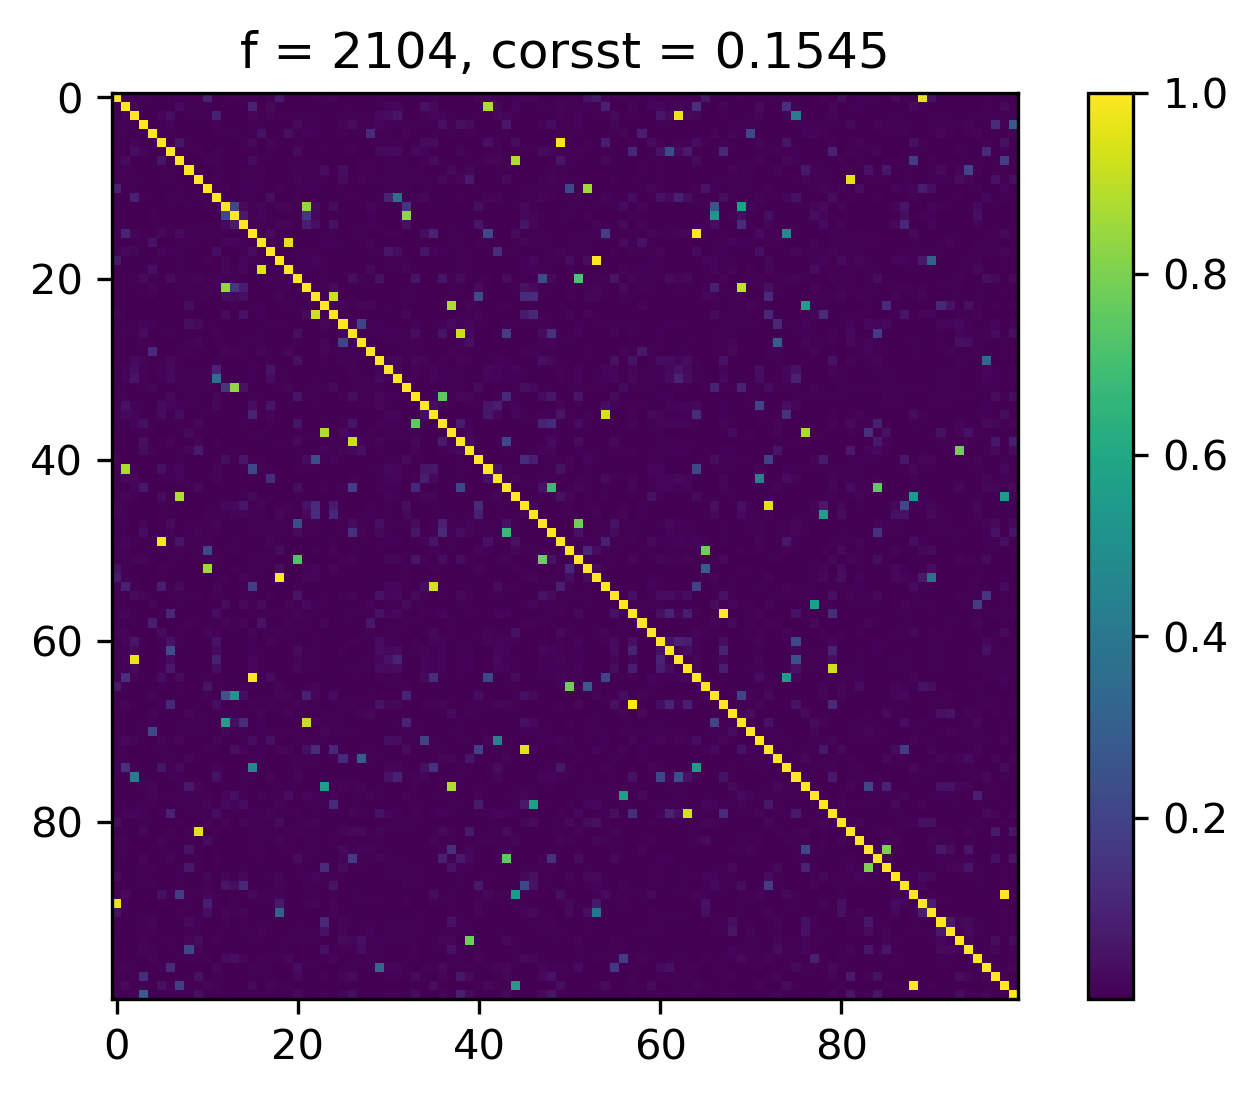
\includegraphics[width=0.9\linewidth]{images/cross5}
			\caption*{Plane wave matrix correlation}
		\end{center}
	\end{minipage}
	\hfill
	\begin{minipage}[c]{.45\linewidth}
		\begin{center}
			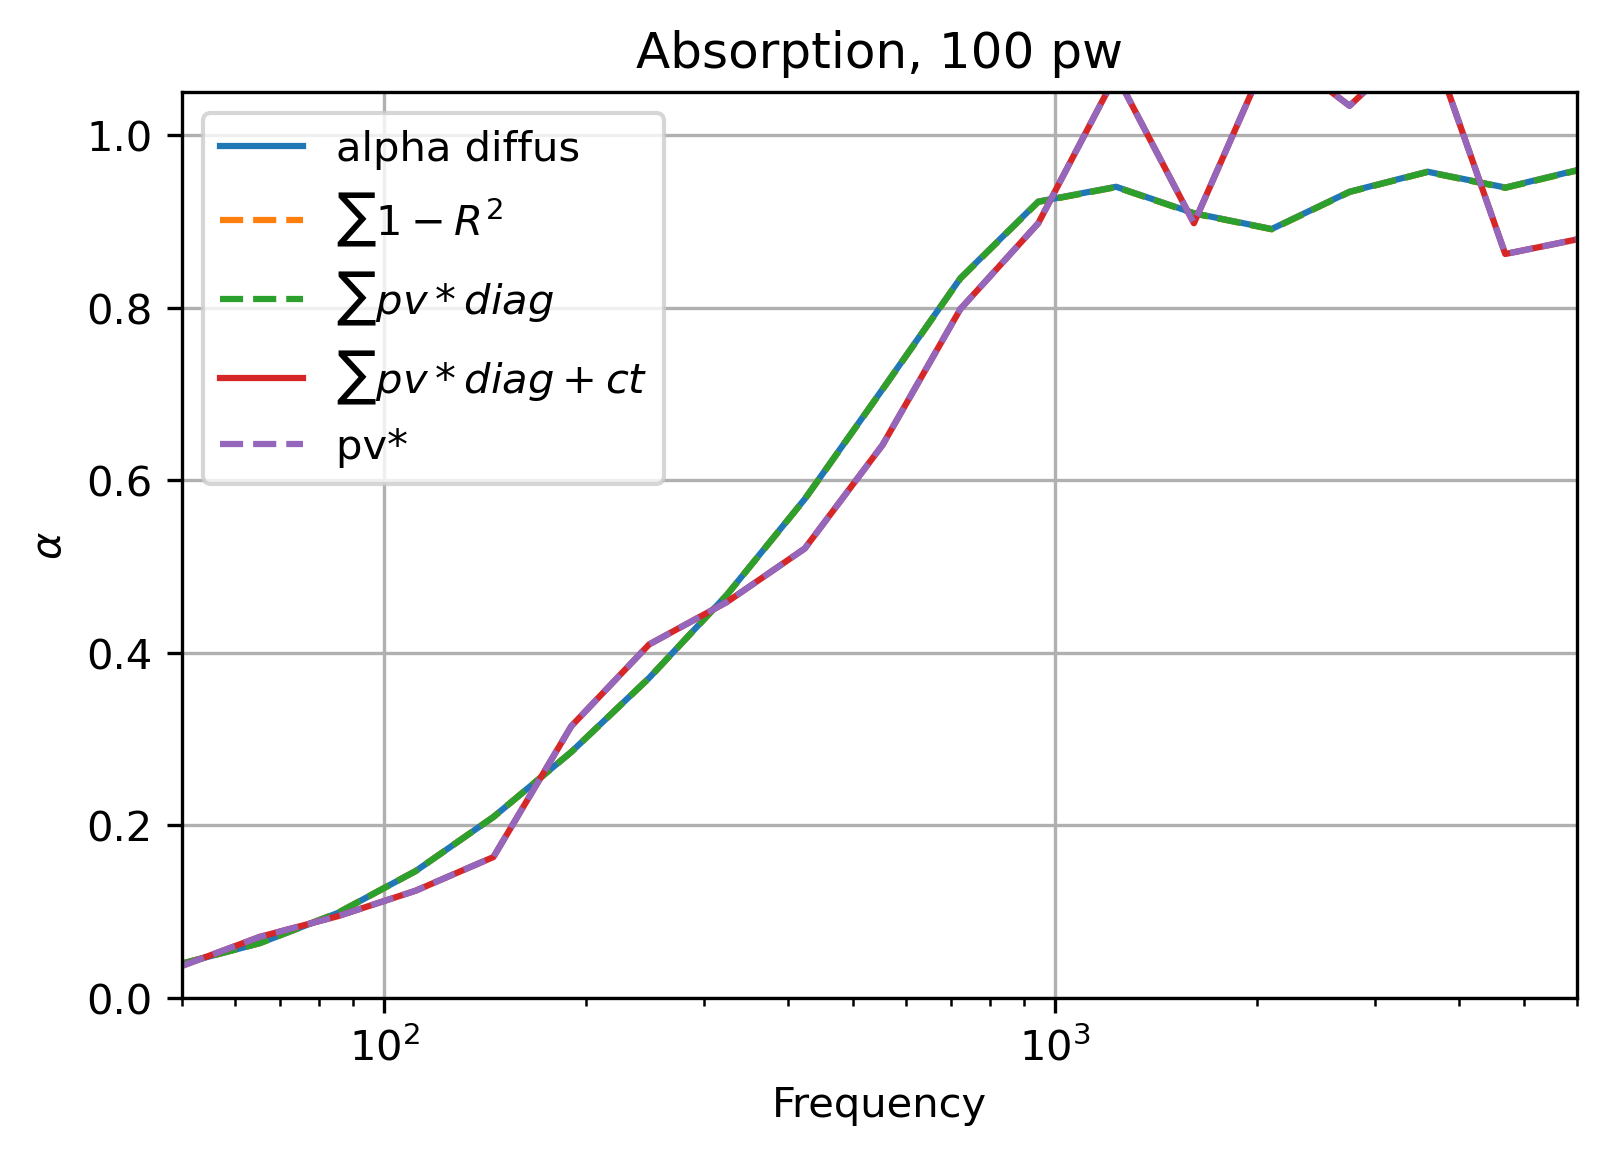
\includegraphics[width=0.9\linewidth]{images/cross6}
			\caption*{Corresponding absorption}
		\end{center}
	\end{minipage}
\end{figure}	

\begin{itemize}
	\item Effet de la zone : petite zone = mauvais spatial averaging : lien avec la taille du sinus cardinal à faire 
	\item Effet du nombre de PW à mieux définir 
\end{itemize}

\section{Optimisation des termes diagonaux pour un plan }
Simulation en plane wave uniquement, sur un plan de microphones pour l'average spatial. La pression et la vitesse sont calculés dessus. Les positions des ondes planes sont optimisées pour réduire la matrice de cross-correlation.\\

\textbf{Proof exemple : }10 PW, 200 Microphones réparties sur une large zone 10000 m ( spatial average)\\
\begin{figure}[h!]
	\centering
	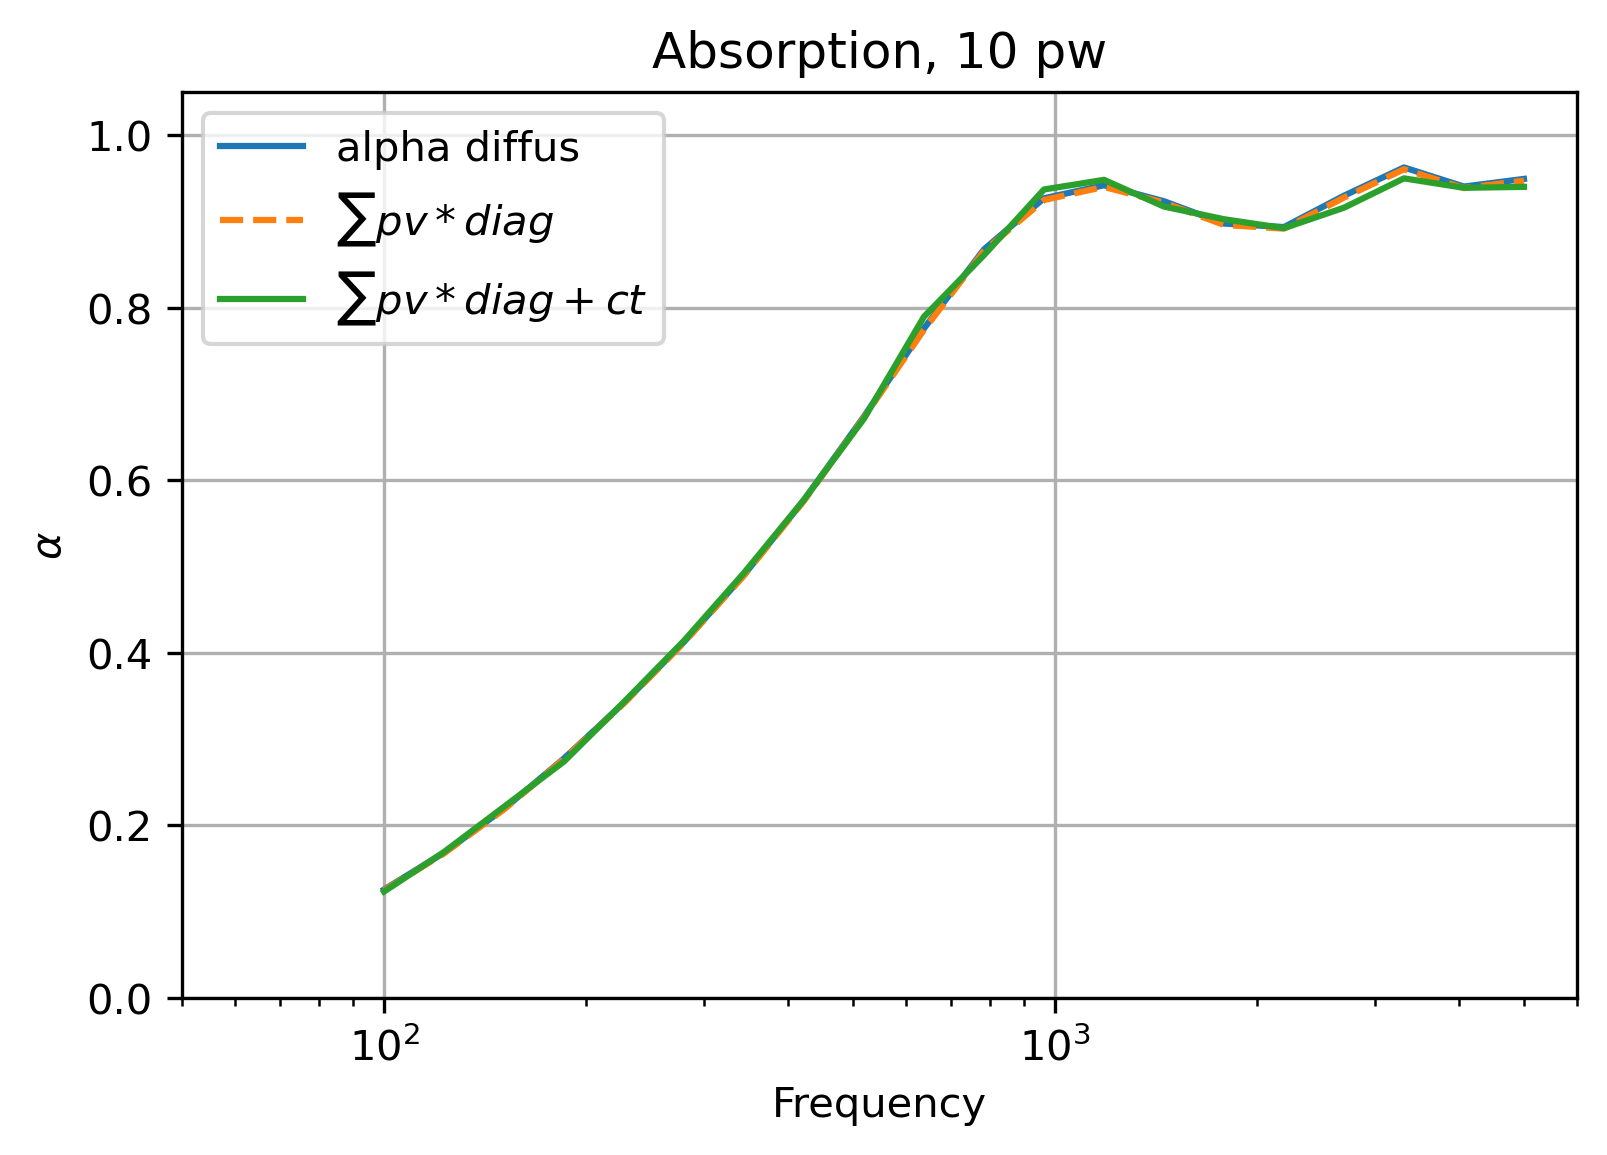
\includegraphics[width=0.7\linewidth]{images/cross7}
	\caption{Absorption avec les position des ondes planes diagonaux optimisés}
	\label{fig:cross7}
\end{figure}

\begin{itemize}
	\item Effet du nombre de PW à mieux définir 
	\item  Mon catch c'est que le plan de microphone pourrait être réduit à un average sur la même position en faisant varier les positions spatiales de l'onde plane (une différente matrice de correlation optimisée à chaque fois) 
\end{itemize}

\section{Conclusion}
\begin{itemize}[label = \textbullet]
	\item Mettre au propre les codes
	\item Mettre au propre la partie rédaction ( Réf manquante ? )
	\item Proof sur un doublet à faire.
	\item Effet des cross terme de réflexion à mieux définir
\end{itemize}


\bibliographystyle{ieeetr}
\bibliography{bib1}


\end{document}
